\chapter{Tests}

\section{Scénario Tests d'acceptation}
% A renommer
Dans un premier temps, l'utilisateur met en place son environnement virtuel. Pour cela, les commandes sont disponibles dans le README.md. 

% a voir si on détaille toutes les commandes pour la générer, mettre une configuration/topologie, détailler topo
Une fois cela effectué, l'utilisateur accède à l'interface de connexion de l'application.

% préciser comment il y accède
L'utilisateur peut s'authentifier avec ses identifiants. Cependant, s'il oublie son mot de passe, il aura la possibilité de le récupérer grâce au lien \textit{Mot de passe oublié ?} situé en dessous de ces deux champs. Imaginons, qu'il l'a effectivement oublié. Il clique donc sur \textit{Mot de passe oublié ?} et une nouvelle fenêtre s'ouvre lui demandant d'entrer son adresse e-mail. Une fois cela fait, il clique sur \textit{Envoyer}. Si tout se passe bien, il devrait recevoir un e-mail avec son mot de passe.

% pas safe à voir
Une fois les deux champs remplis, l'utilisateur clique sur \textit{Log In}. Maintenant, l'utilisateur est redirigé vers l'interface de l'application lui permettant d'exécuter différentes actions. 

La premier chose que l'utilisateur voit est le voyant, attestant de la bonne ou mauvaise fonctionnalité. Le voyant étant vert, l'application fonctionne.

% détailler si le voyant est rouge.
Ensuite, il peut attester de son identité et voit tous ses réseaux.

Il a précédemment remarqué qu'un trafic trop important se dirigeait vers l'un de ses serveurs. 

Après étude, il en ressort l'adresse IP attaquante et l'adresse IP cible. A ce stade, il y a trois choix possibles. Soit l'utilisateur décide de router par source, par destination ou par communautés. Nous allons étudier ces trois cas.

Il va donc neutraliser l'attaquant en changeant le routage vers la cible. Il veut maintenant ajouter une route pour rediriger l'attaque vers un trou noir. Dans le champs \textit{IP ou réseau}, il renseigne l'adresse attaquante. Dans \textit{Prochain saut}, il renseigne le prochain saut vers un trou noir, sachant qu'il a le droit à une liste. Ensuite, il peut sélectionner la ou les communautés à laquelle il veut appliquer cette modification. Une fois cela fait, il peut cliquer sur \textit{Valider}.

A ce moment, une requête HTTP est envoyé de l'interface utilisateur vers l'API. Celle-ci envoie une requête à ExaBGP. ExaBGP va donc diffuser la nouvelle route sur le réseau. Une fois cela effectué, ExaBGP envoie une réponse à l'API. Deux cas sont donc possibles : la diffusion a réussi ou elle a échoué. 

Prenons le cas de la réussite. L'API va donc mettre à jour la base de données. Cela fait, l'utilisateur verra apparaître le changement sur son interface.

Si la diffusion de la route échoue, l'API ne modifiera pas la base de données. Elle enverra une requête à l'interface utilisateur qui affichera un message d'erreur.

Quelques temps plus tard, le trafic semble s'être réduit. L'utilisateur a donc deux choix possibles : Supprimer la route qu'il a précédemment créé ou tout simplement la désactiver.

Commençons par cette seconde option. L'utilisateur, ne sait pas si le problème reviendra plus tard. Il décide donc de désactiver la route précédemment créée. Les informations seront toujours contenues dans la base de données. Cela lui évitera de la saisir de nouveau. Il va donc sélectionner la route et cliquer pour la désactiver. Une requête est donc envoyée à l'API qui va elle-même en envoyer une a ExaBGP pour diffuser le nouveau message sur les routeurs et la route n'existera donc plus sur la table de routage de ceux-ci. Après avoir reçu la réponse d'ExaBGP, l'API va mettre à jour la base de données de la même manière qu'expliquée précédemment. La route sera toujours présente dans la base de données. 

Prenons maintenant la deuxième option. L'utilisateur sélectionne simplement la route précédemment créée et clique pour la supprimer. Une requête est envoyée à l'API, et de la même manière que la désactivation une diffusion est envoyée aux routeurs et la routes n'existe donc plus sur la table de routage de ceux-ci, ni sur la base de données. \\ \indent
Il y a de nouveau une attaque venant de la même adresse IP. Si l'utilisateur a supprimé la route, il est obligé de la créer de nouveau. S'il l'a désactivée, il n'aura qu'à la sélectionner et l'activer.

Dans ce deuxième cas, il va générer un routage par destination. Tout le trafic se dirigeant vers son serveur sera redirigé vers un trou noir. 

%détailler par dest


%détailler par communautés
Dans le cas ou l'utilisateur souhaite faire un routage par communauté, il pourra diffuser une demande de routage qui s'appliquera à tout les membres de la communauté sans s'appliquer aux autres.

L'utilisateur souhaite maintenant quitter sa session. Il clique sur son identité. Un bouton \textit{Déconnexion} apparaît. Il clique dessus. L'utilisateur est redirigé sur l'interface de connexion. Il ne peut plus rien faire sauf entrer ses identifiants de nouveau ou faire une demande suite à l'oubli de son mot de passe.


% Test de performances
\begin{figure}[H]
    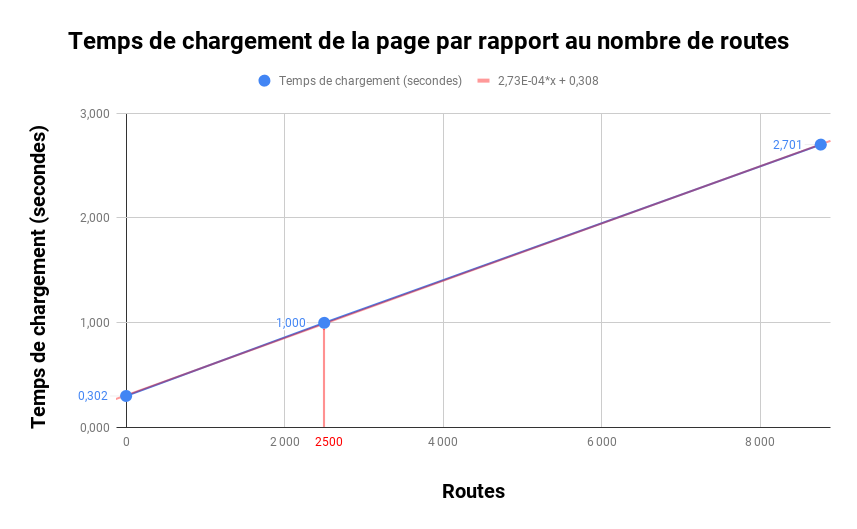
\includegraphics[width=\textwidth]{small_scale.png}
    \caption{Diagramme d'utilisation de l'application}
    \label{fig:use_cases}
\end{figure}

\begin{figure}[H]
    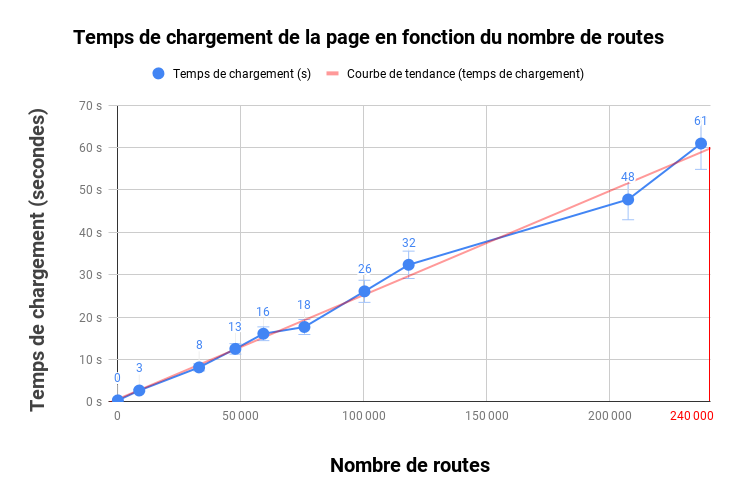
\includegraphics[width=\textwidth]{big_scale.png}
    \caption{Diagramme d'utilisation de l'application}
    \label{fig:use_cases}
\end{figure}

% Graph : 2.500 routes en une seconde
% Graph : 240.000 routes en une minute


% Tests d'authentification
% Tests d'API
% Test frontend (form)

